%*******10********20********30********40********50********60********70********80
\chap{Background Theory}

What the reader needs to know in order to understand the rest of the report. Examiners like to know that you have done some background research and that you know what else has been done in the field (where relevant). Try to include some references.
    Related work (if you know of any)
    What problem are you solving?
    Why are you solving it?
    How does this relate to other work in this area?
    What work does it build on?
    
\section{Agile Software Development}

\section{Ruby on Rails} 
Ruby on Rails, or simply Rails, is a server-side web application framework written in Ruby under the MIT License. Rails is a model–view–controller (MVC) framework, providing default structures for a database, a web service, and web pages. It encourages and facilitates the use of web standards such as JSON or XML for data transfer, and HTML, CSS and JavaScript for display and user interfacing. In addition to MVC, Rails emphasizes the use of other well-known software engineering patterns and paradigms, including convention over configuration (CoC), don't repeat yourself (DRY), and the active record pattern. \cite{wiki:RoR}
\begin{figure}[H]
	\centering
    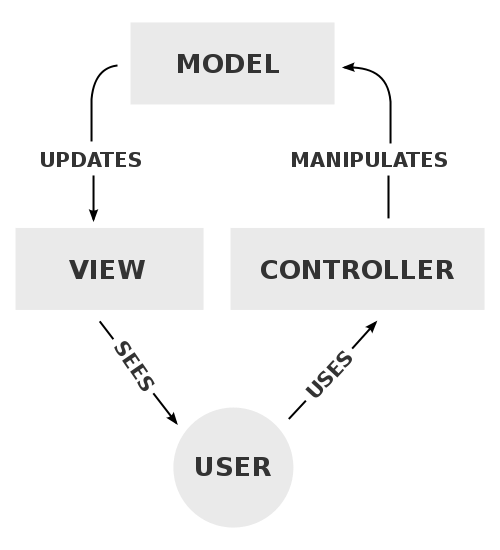
\includegraphics[trim={0 0 0 0},clip,width=0.7\textwidth]{Files/MVC.png}
    \caption{Diagram of interactions within the MVC pattern.\\ \textbf{Source:} https://en.wikipedia.org/wiki/Model-view-controller}
    \label{fig: MVC}
\end{figure}


